Das zwölfwöchige Pflichtpraktikum wurde in der Abteilung ADAS Driving Functions/ Chauffeur Functions der Firma Continental Teves AG \& Co. oHG in Eschborn absolviert. Im Folgenden wird zu Beginn eine Übersicht der Tätigkeitsfelder der Abteilung, in welcher das Praktikum unter Bearbeitung interdisziplinärer Tätigkeitsfelder absolviert wurde, gegeben, bevor darauf folgend die Aufgaben und Tätigkeiten, welche während des Praktikums bearbeitet wurden, beschrieben werden. 

Die Abteilung ist im Bereich des automatisierten Fahrens tätig. Das automatisierte Fahren lässt sich hierbei nach SAE-Standard J3016 in insgesamt fünf Automatisierungsgrade unterteilen. Beschreibt der Automatisierungsgrad des Levels 0 einen Zustand, in dem der Fahrer selbst fährt und im Zuge dessen alle Manöver wie Beschleinigung oder Bremsung selbst durchführt, so handelt es sich bei dem Automatisierungsgrad des Level 5 um einen komplett autonomen Zustand, in welchem der Fahrer keinerlei Beitrag zum Kontrollieren des Fahrzeugs leistet, außer die Vorgabe des Fahrziels sowie des Starten des Systems [Quelle: xxx]. Die Abteilung, in welcher das Pflichtpraktikum absolviert wurde, ist in diesem Kontext innerhalb des Automatisierungsgrades Level 2+ anzusiedeln. Funktionen wie automatisches Einparken, Spurhalten, Abbremsen auf andere Verkehrsteilnehmer sind hier im Fahrzeug integriert. Ebenso sind Fahrfunktionen wie ACC (Adaptive Cruise Control), welches einen konstanten Abstand zu vor dem eigenen Fahrzeug befindlichen Verkehrsteilnehmern in Abhängigkeit ihrer Geschwindigkeiten einhält. Ein besonderer Arbeitsschwerpunkt der Abteilung liegt auf dem automatisierten Spurwechsel, welcher laut SAE-Standard J3016 formell im Automatisierungsgrad Level 3 anzuordnen ist.

Praktikumstätigkeiten
Der erste Einsatzbereich fand im Bereich des automatisierten Spurwechsels im High-Way-Kontext, also auf der Autobahn, statt. Im Folgenden wird die ebenfalls in der Abteilung verwendete Fachsprache benutzt, die verwendeten Abkürzungen werden bei der ersten Erwähnung erläutert und finden sich des Weiteren im Abkürzungsverzeichnis dieses Berichtes (siehe Abkürzungsverzeichnis). Das Vehikel, für welches die automatisierten Funktionen implementiert werden sollen, wird als Ego bezeichnet. Andere Verkehrsteilnehmer werden mit TPO (Traffic Participant Object) gekennzeichnet. Eine Fahrspur wird mit dem Begriff Lane betitelt, die die Lane jeweils nach rechts und links begrenzenden Fahrbahnmarkierungen entsprechend mit Lane-Marker. Die Fahrspur, auf dem sich das Ego-Fahrzeug aktuell befindet, wird mit Ego-Lane bezeichnet. Im Kontext eines geplanten Fahrspurwechsels erhält die Fahrspur, die als Ergebnis des Spurwechsels dient, den Namen Target-Lane. Das erste betrachtete Szenario umfasst ein Ego-Fahrzeug, welches sich zum Startzeitpunkt auf der rechten Spur einer zweispurigen Autobahn befindet. Vor dem Ego-Fahrzeug befindet sich auf der rechten Spur ein TPO. Der Set-Speed, also die gewollte Geschwindigkeit, beträgt 100 km/h. Da das TPO auf der Ego-Lane jedoch nur eine Geschwindigkeit von 80 km/h vorweist, fährt das Ego mit aktiviertem ACC mit konstantem Abstand hinter dem TPO her. Auf der Target-Lane befindet sich ebenfalls ein TPO, welches mit konstanten 80 km/h fährt. Der Wunsch eines Fahrspurwechsels wird, wie bereits erwähnt, durch das Setzen des Blinkers in die gewünschte Richtung signalisiert. Darauf folgend wird unter zu Hilfe nahme der Umgebung eine abzufahrende Bahn geplant. Da diese Bahn keine visuellen Informationen bereitstellt, erfolgte eine solche Visualisierung in einem ersten Schritt innerhalb des Praktikums. Mittels der Programmiersprache Python wurde das anfangs beschriebene High-Way-Szenarion simuliert und visualisert. Ein erstes Konzept der Visualisierung ist in Abbildung xy zu sehen. 

\begin{figure}[!ht]
	\begin{center}
		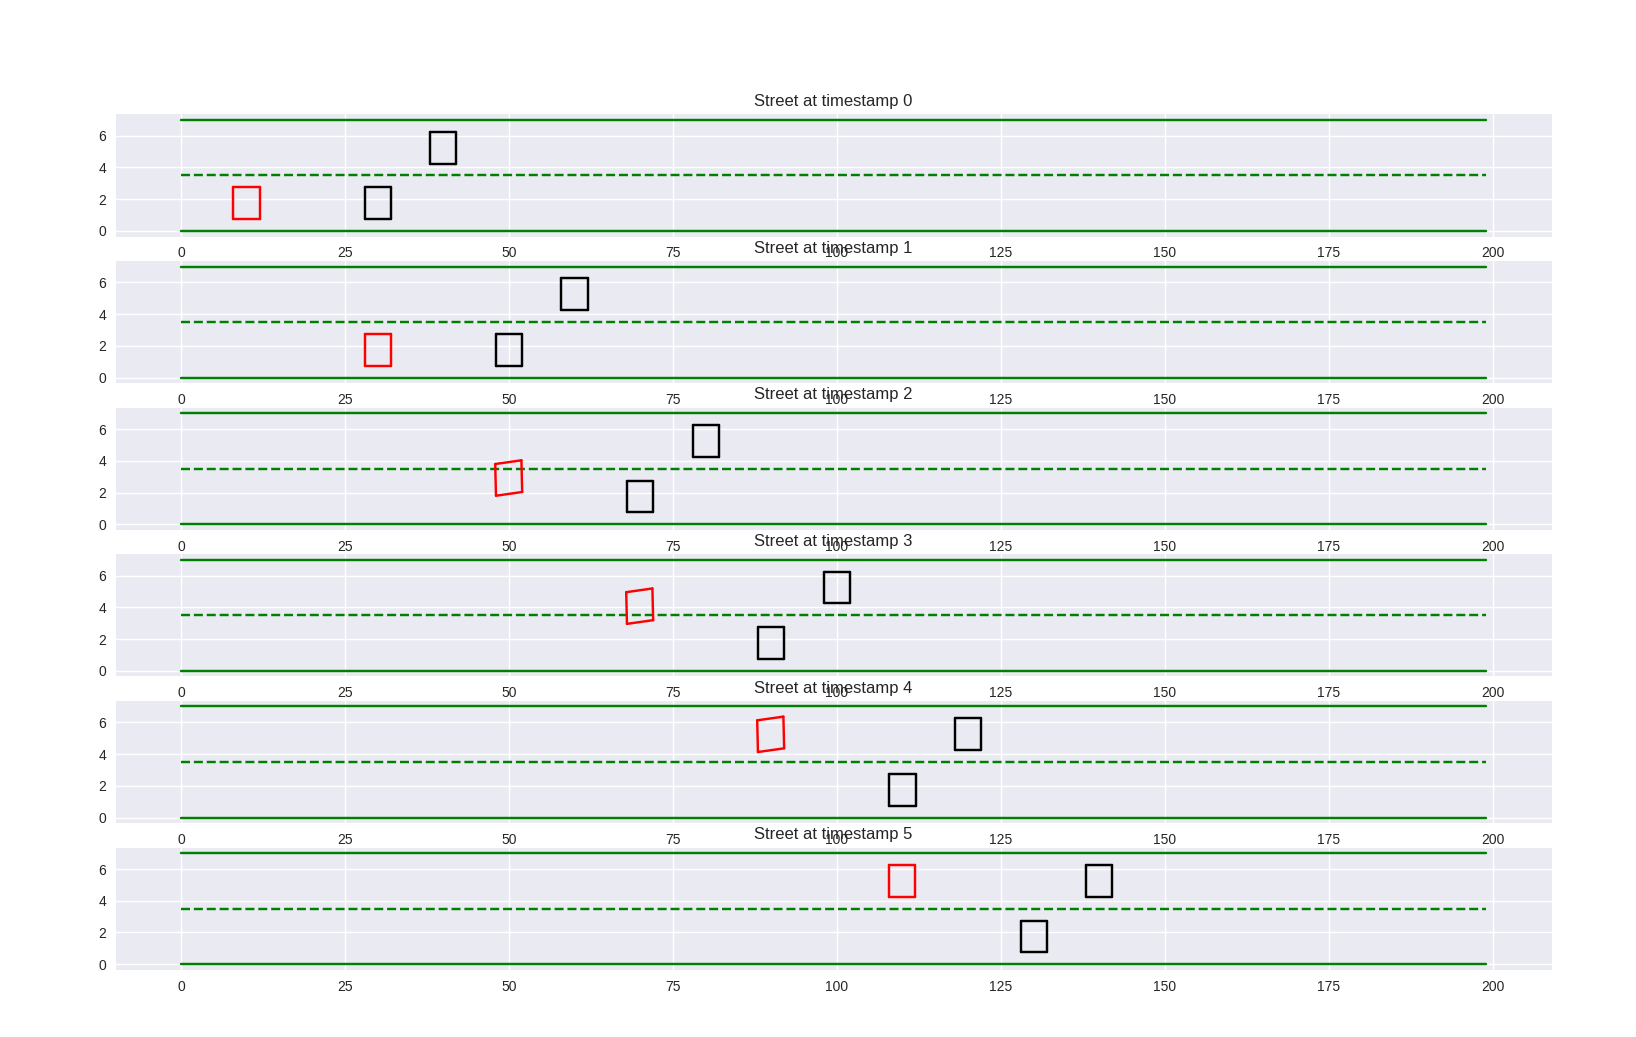
\includegraphics[width=0.8\linewidth]{Abbildungen/bericht/lanechange_visualization}
		\caption{Visualisierung Highway-Spurwechsel in Python}
		\label{fig.highway_spurwechsel_python}
	\end{center}
\end{figure} 

In rot dargestellt sind hier die schemenhaften Umrisse des Ego-Fahrzeuges, in schwarz dargestellt sind die TPO's auf der Ego-Lane sowie auf der Target-Lane. Über mehrere Zeitschritte hinweg ist die Veränderung der Position sowie der Orientierung der Verkehrsteilnehmer während des Spurwechsels aufgetragen. Die Lane-Marker sind im Diagramm in grün eingezeichnet. 
In einem nächsten Schritt erfolgte die Portierung des Visualisierungskonzeptes von der Programmiersprache Python in die Programmiersprache C++. Diese Portierung wurde durch die Tatsache, dass die Planungsalgorithmen für den Spurwechsel ebenfalls in C++ geschrieben sind.

% Kann man hier ggf noch ein Bild von der Gesamtübersicht reinpacken, wie z.B. von dem Eingang der Sensordaten etc? Frank fragen.

Ein weiterer Grund für die Portierung ergibt sich daraus, dass die Datentypen, welche in der urpsprünglichen Python-Visualisierung noch selbst erstellt waren, nun auf die von den tatsächlichen Algorithmen verwendeten Datentypen angepasst werden mussten. Bild xy stellt die fertige Visualisierung dar, der Übersichtlichkeit halber sind nur zehn Zeitschritte des Spurwechsels dargestellt. Im Gegensatz zu Bild xy ist die C++ - Portierung um einige Funktionalitäten ergänzt.
